\begin{figure}[htpb]
	\centering\capstart{}
	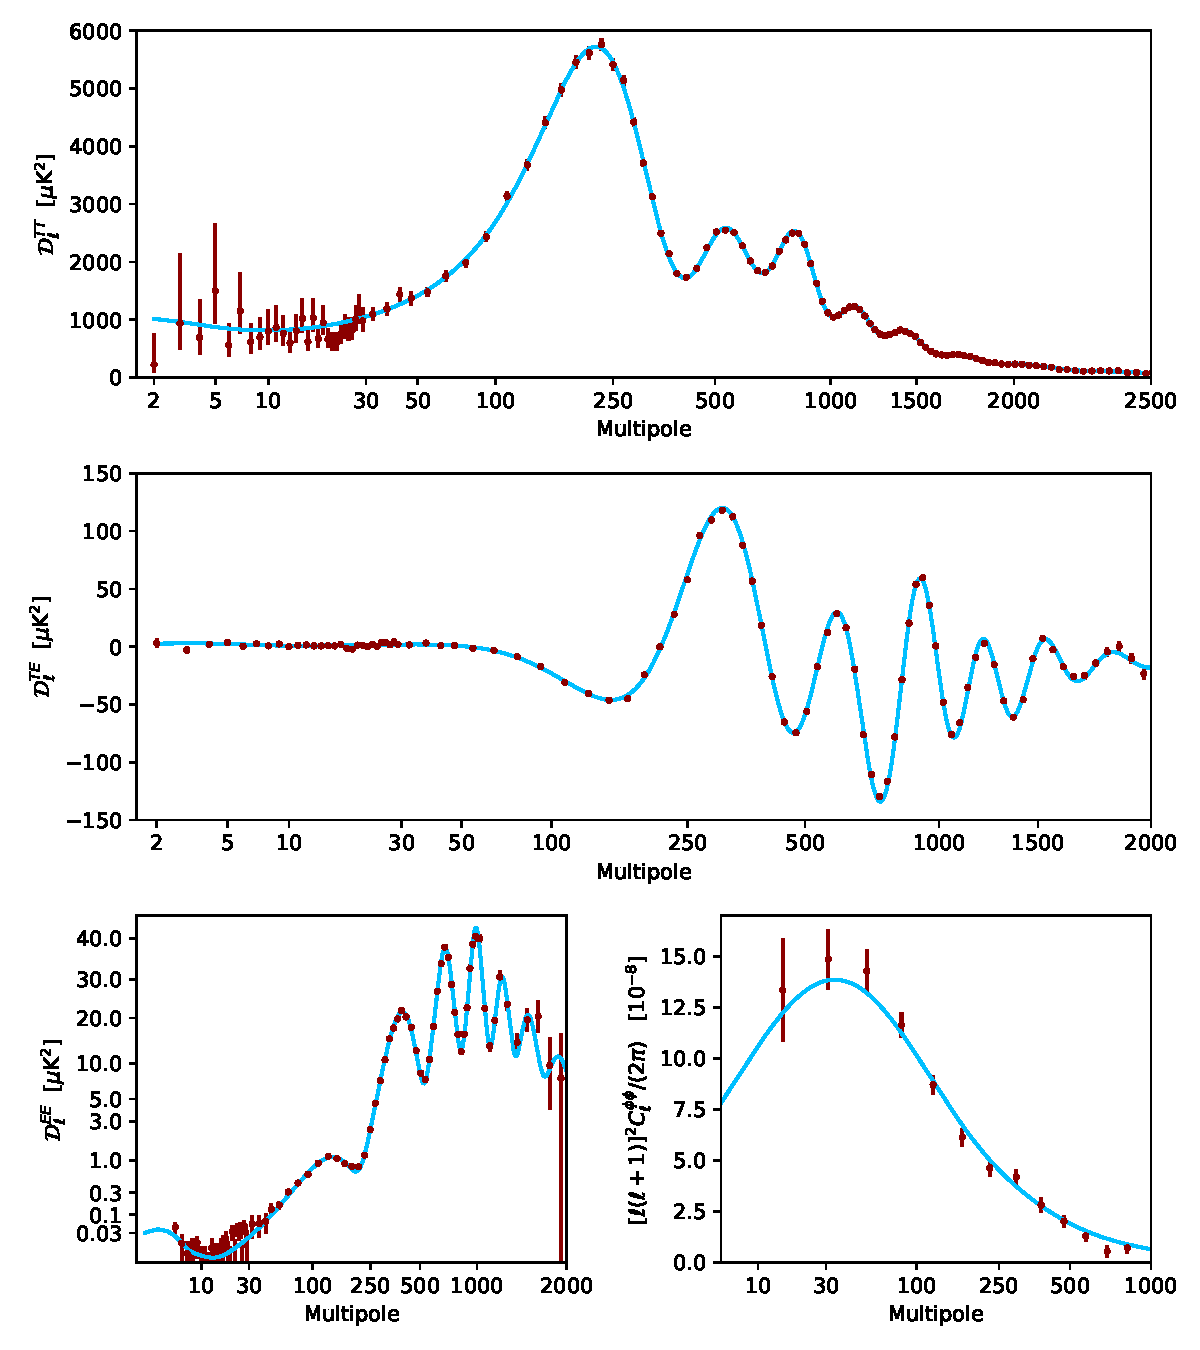
\includegraphics[trim={0 430 0 0},clip,width=\textwidth]{planck_2018_power_spectrum.pdf}
	\caption[
	The 2018 Planck CMB angular power spectrum in temperature
	]{
	Measurements of the angular power spectrum of the Planck CMB temperature anisotropies (in red), where \(D_{\ell} = \ell(\ell+1)C_{\ell}/2\pi{}\) (courtesy of The Planck Collaboration 2018~\cite{Planck2020}).
	The spectrum is often plotted for \(D_{\ell}\) rather than \(\powerSpectrum{}\) as this gives a flat Sachs-Wolfe plateau for low \(\ell{}\) on a logarithmic scale.
	The blue line is a best-fit model to temperature and polarisation data.
	The error bars at low-\(\ell{}\) are dominated by cosmic variance.
	}\label{fig:chapter2_power_spectrum}
\end{figure}
